\chapter{Projeto de Solução}

Com base nos requisitos então elicitados, pôde-se ter uma noção clara de como seria feita a implementação da aplicação e este processo teve início. Ao longo dele, \textit{feedback} a respeito da estética da ferramenta foi constantemente colhido com a equipe de desenvolvedores da empresa júnior, bem como de parceiros do grupo de pesquisa do qual o autor faz parte.

O intuito da ferramenta é permitir a criação de documento que vinculem recursos de repositórios no GitHub (arquivos, \textit{commits} e \textit{pull requests}), bem como outros referenciais (\textit{links} para perguntas no Stack Overflow, tutoriais ou \textit{blogs}, por exemplo) de forma a gerar um guia ou tutorial de como realizar tal implementação novamente no futuro. Dentro da ferramenta, um documento é chamado de twydi.

A ferramenta é de código livre e uma versão em execução pode ser acessada utilizada por qualquer desenvolvedor\footnote{\url{http://that-s-the-way-you-do-it.herokuapp.com}}. Informações sobre licensa e o código da ferramenta podem ser encontradas em seu repositório público\footnote{\url{https://github.com/coopera/that-s-the-way-you-do-it}}.

\section{Listagem de Documentos}

Na tela inicial da aplicação é possível ver uma lista com todos os documentos já criados. Cada documento é exibido com seu título, descrição, lista de \textit{tags} e autor (caso tenha se identificado durante a criação do documento), conforme apresentado nas figuras \ref{fig:doc-list-1} e \ref{fig:doc-list-2}.

\begin{figure}[h!]
	\centering
    \caption{Listagem de Documentos}
    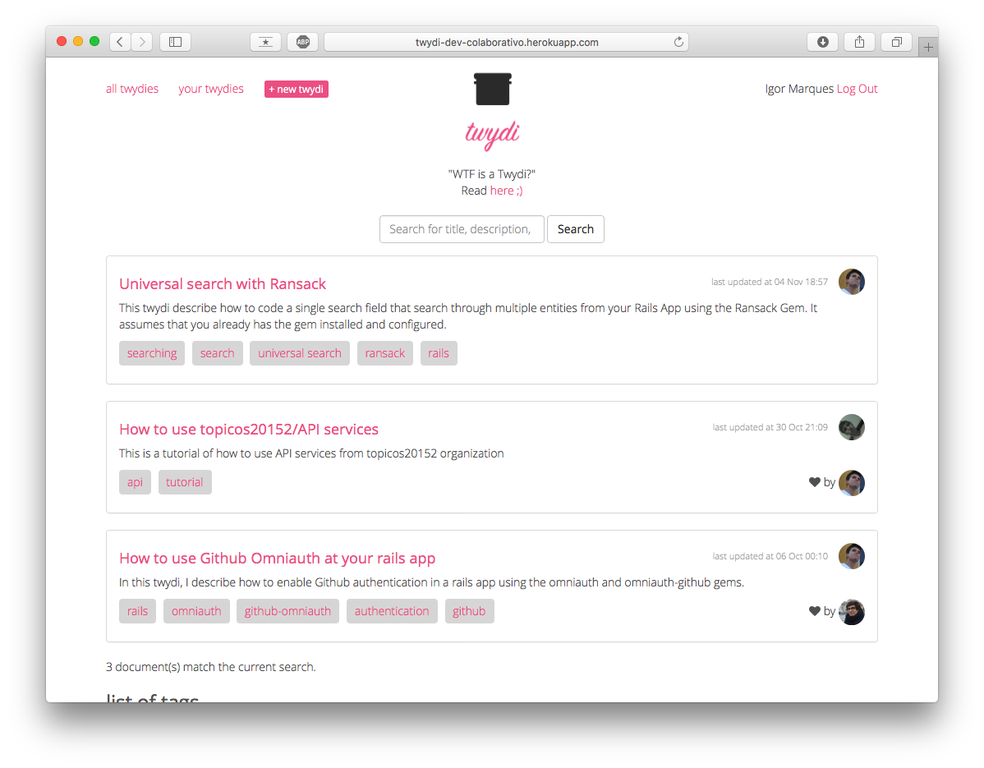
\includegraphics[width=15cm]{Imagens/print-lista-1.png}
		\label{fig:doc-list-1}
	\caption*{Fonte: O autor (2015)}
\end{figure}

\begin{figure}[h!]
	\centering
    \caption{Listagem de Documentos (parte inferior da página)}
		\label{fig:doc-list-2}
    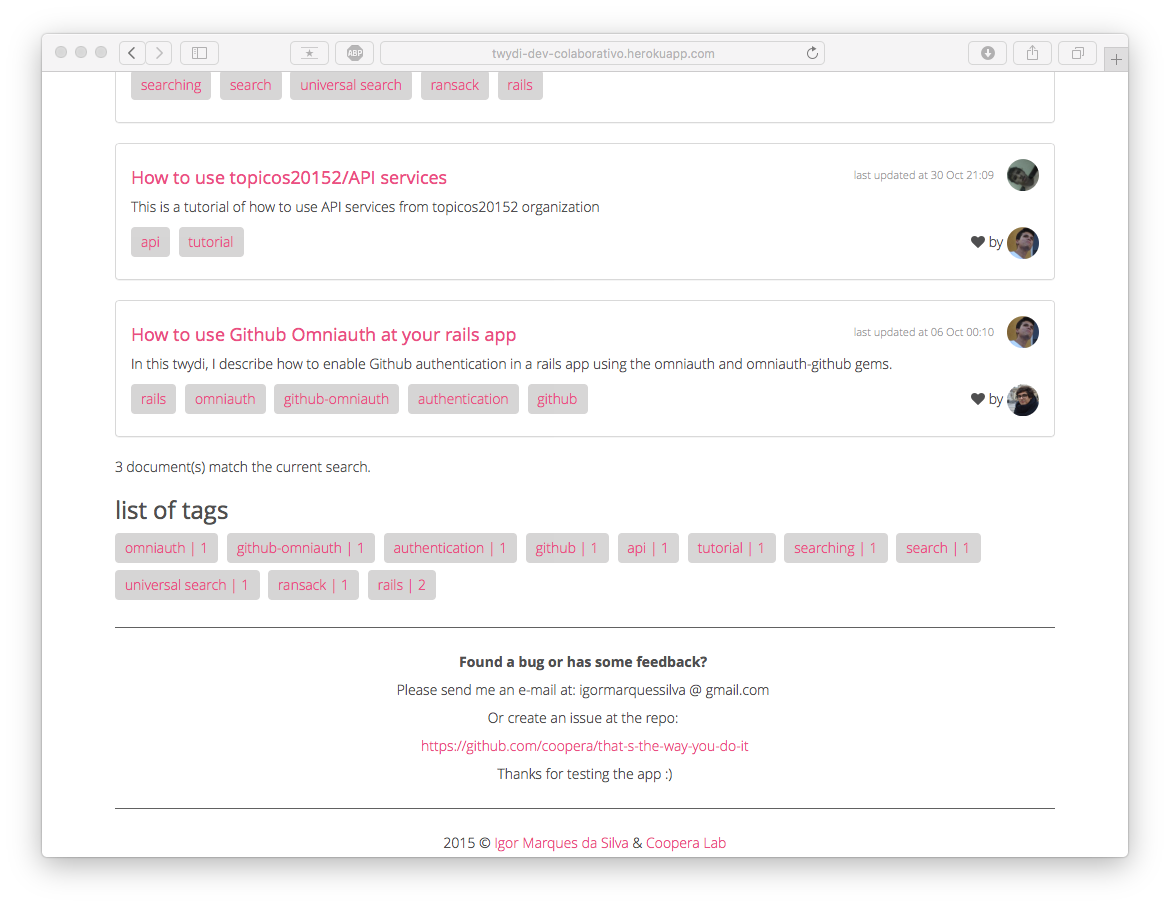
\includegraphics[width=15cm]{Imagens/print-lista-2.png}
	\caption*{Fonte: O autor (2015)}
\end{figure}

Ao fim da lista de documentos, é possível ver quantos documentos se encontram nela e também uma lista das \textit{tags} presentes, incluindo sua quantidade de ocorrências dentro do grupo de documentos exibidos, como pode ser visto na figura \ref{fig:doc-tags}.

\begin{figure}[h!]
	\centering
    \caption{Lista de \textit{tags}}
    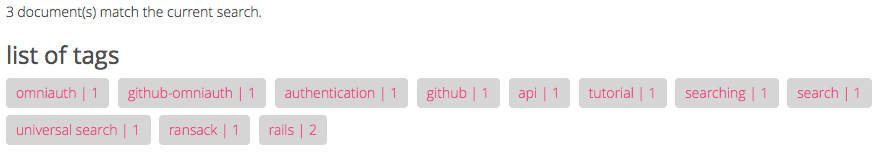
\includegraphics[width=15cm]{Imagens/print-tags.png}
		\label{fig:doc-tags}
	\caption*{Fonte: O autor (2015)}
\end{figure}


\section{Criação de um Documento}

Qualquer usuário da aplicação pode criar um documento, mesmo sem estar autenticado na mesma. A figura \ref{fig:doc-new} mostra a tela de criação de um documento.
% IM: tá ruim esse parágrafo, eu sei.

\begin{figure}[h!]
	\centering
    \caption{Novo documento}
    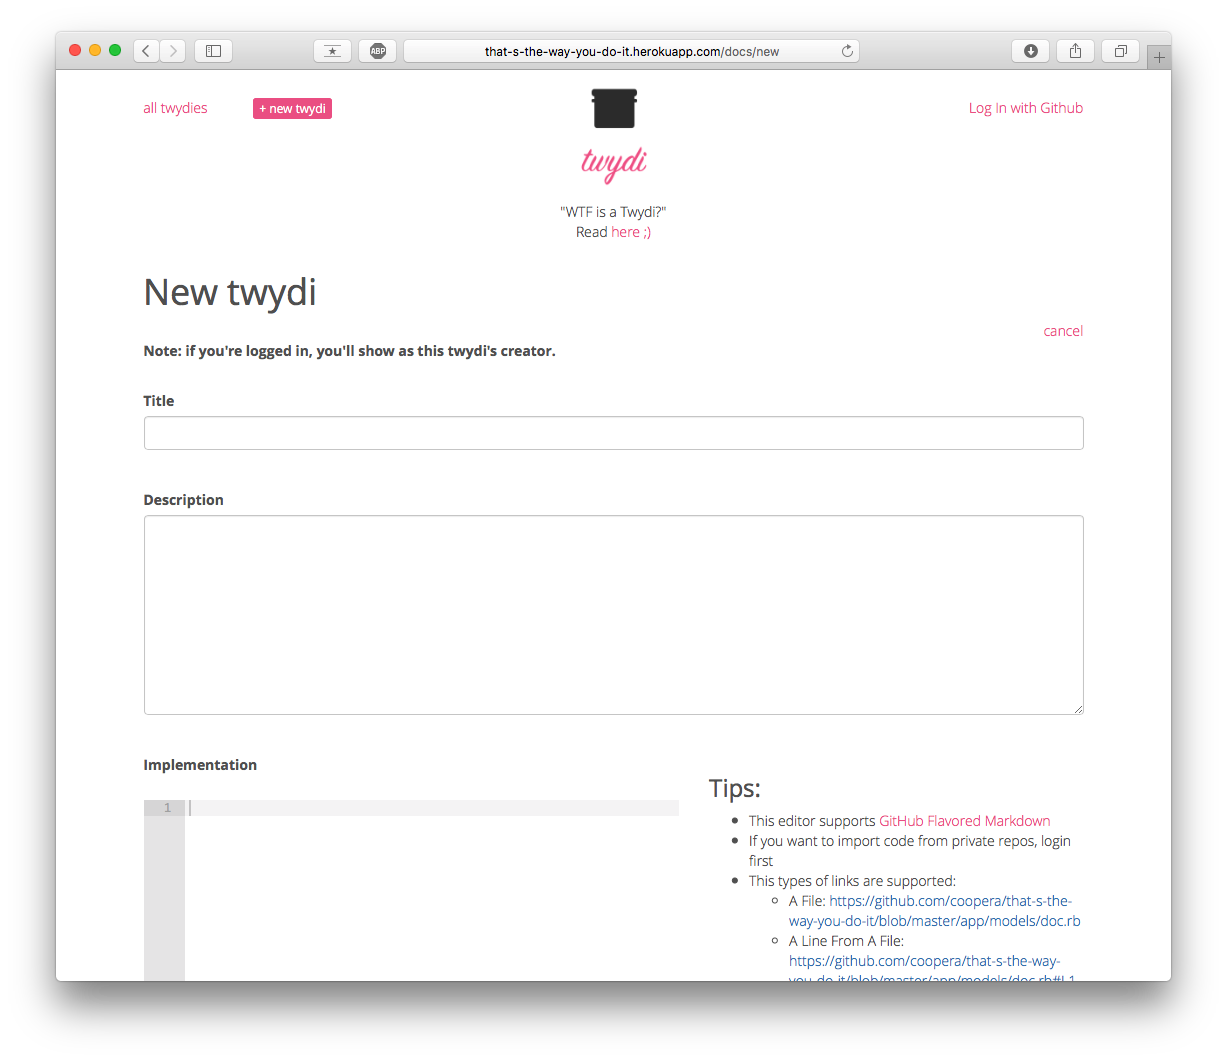
\includegraphics[width=15cm]{Imagens/print-new-twydi.png}
		\label{fig:doc-new}
	\caption*{Fonte: O autor (2015)}
\end{figure}

\subsection{Elementos de um documento}

Um documento é composto por 5 elementos, todos informados pelo seu autor:

\begin{itemize}
  \item Título: Título do documento. Deve fornecer uma noção sobre o que aquele documento descreve.
  \item Descrição: Um resumo sobre o que o documento descreve. Descritivo o suficiente para que outros usuários não tenham que ler o documento inteiro para compreender sobre o que ele trata.
  \item Implementação: Procedimento sobre como implementar ou executar a funcionalidade descrita. Possui suporte a linguagem de marcação e importação de código armazenado em repositórios públicos e privados do GitHub.
   \item \textit{Links} Relacionados: Lista de \textit{links} relevantes para o documento, cada um com descrição própria. Podem conter referências utilizadas para elaborar o documento ou material mais avançado sobre o assunto.
  \item \textit{Tags}: Lista de \textit{tags} sobre o assunto do documento. Utilizada para facilitar sua recuperação posteriormente tanto pelo autor quanto por outros usuários.
\end{itemize}

Sobre o elemento Implementação, a próxima subseção o descreve em detalhes.

\subsection{Implementação}

Elemento mais relevante de um documento e é utilizado para que o usuário descreva um passo-a-passo sobre como realizar a implementação de uma funciondalidade, ou deixe registrado determinado procedimento. Dentre suas funcionalidades que permitem um uso aprimorado por parte de equipes de desenvolvimento de software está a importação de código hospedado no GitHub.

No GitHub é possível acessar cada arquivo de um determinado projeto através de URLs simples e que seguem a própria estrutura de diretórios do projeto em em questão.

Por exemplo, um arquivo com caminho ``app/models/example.rb'' se encontra URL ``github.com/usuario/projeto/blob/master/app/models/example.rb''.

O arquivo é exibido utilizando uma formatação própria da linguagem, facilitando sua visualização. Um exemplo pode ser visto na figura \ref{fig:doc-show-show}.

\begin{figure}[h!]
	\centering
    \caption{Exibição de documento}
    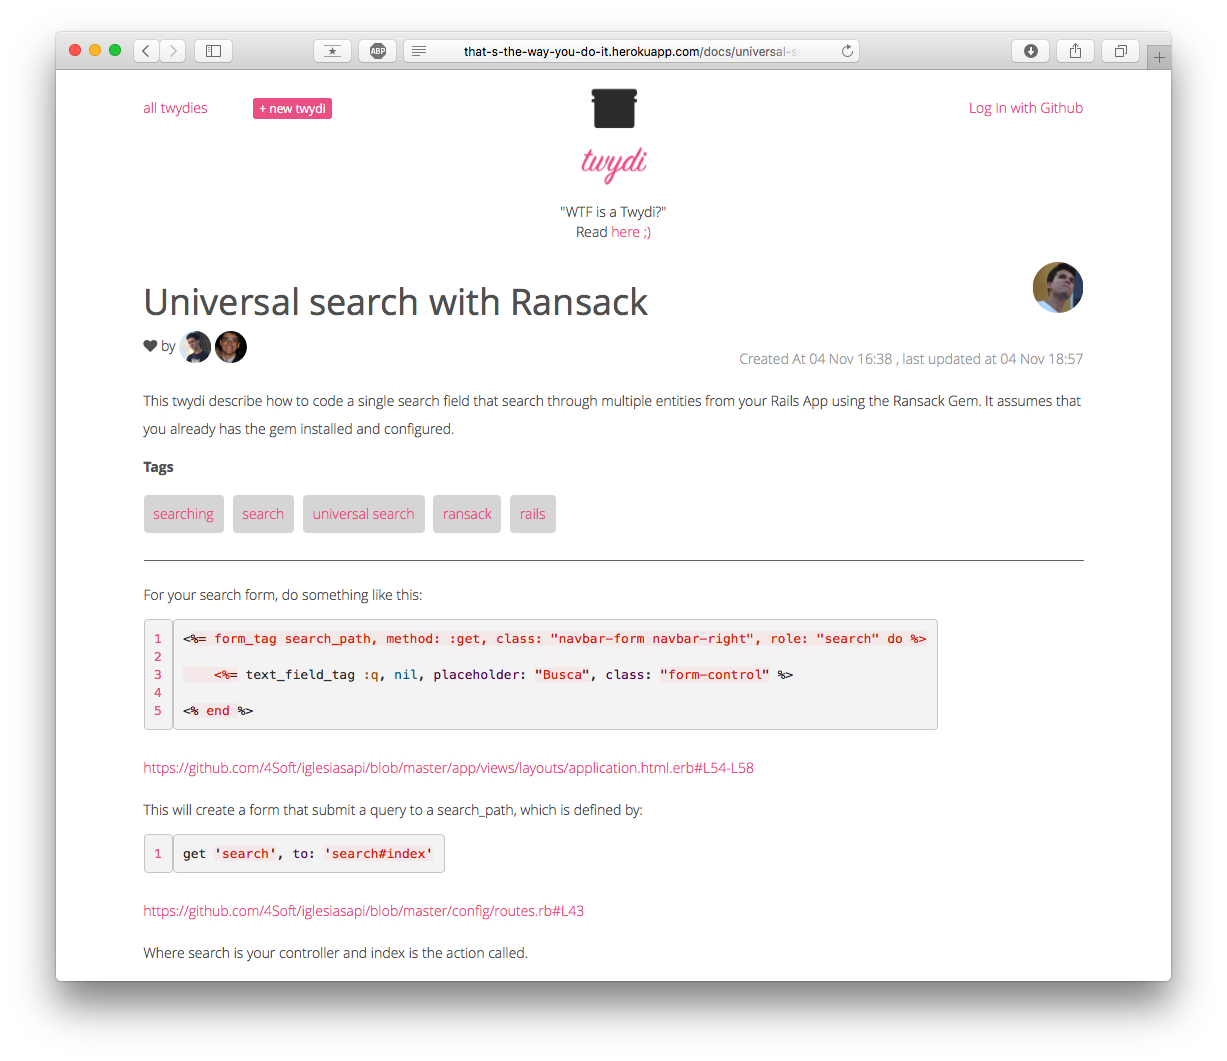
\includegraphics[width=15cm]{Imagens/print-implementation-1.png}
		\label{fig:doc-show-show}
	\caption*{Fonte: O autor (2015)}
\end{figure}

A partir dessa estrutura de URLs, foi elaborado um mecanismo para importar código no editor de texto da implementação toda vez que um \textit{link} do GitHub é colado. Uma descrição sobre os tipos de importações possíveis e seus respectivos resultados encontra-se na Tabela 2.

\begin{table}[]
\centering
    \caption{Tipos de importação suportadas pela aplicação}
    \label{my-label}
    \begin{tabular}{p{3cm} | p{7cm} | p{5cm}}
    \hline
    Tipo da Importação & Exemplo de link & Resultado \\ \hline
    Arquivo & \url{https://github.com/coopera/that-s-the-way-you-do-it/blob/master/app/models/doc.rb} & Conteúdo Inteiro do Arquivo é importado. \\ \hline
    Linha de Arquivo & \url{https://github.com/coopera/that-s-the-way-you-do-it/blob/master/app/models/doc.rb\#L1} & Apenas a linha informada é importada. \\ \hline
    Intervalo de Linhas de Arquivo & \url{https://github.com/coopera/that-s-the-way-you-do-it/blob/master/app/models/doc.rb\#L5-L7} & O conteúdo intervalo entre as inclusivo entre linhas é importado. \\ \hline
    \textit{Commit} & \url{https://github.com/coopera/that-s-the-way-you-do-it/commit/d7f365db9777b4cb6e1c5799}
    \url{a2e431c58aaf3a19} & Um \textit{diff} contendo o conteúdo adicionado e removido no \textit{commit} é importado. \\ \hline
    \textit{Pull Request} & \url{https://github.com/coopera/that-s-the-way-you-do-it/pull/7} & Um \textit{diff} contendo o conteúdo adicionado e removido em todos os \textit{commits} do \textit{pull request} é importado.  \\ \hline
\end{tabular}
\caption*{Fonte: O autor}
\end{table}

Exemplos dos resultados de cada importação podem ser vistos nas figuras \ref{fig:doc-import-1}, \ref{fig:doc-import-2}, \ref{fig:doc-import-3} e \ref{fig:doc-import-4}.
\begin{figure}[h!]
	\centering
    \caption{Importação de Arquivo}
    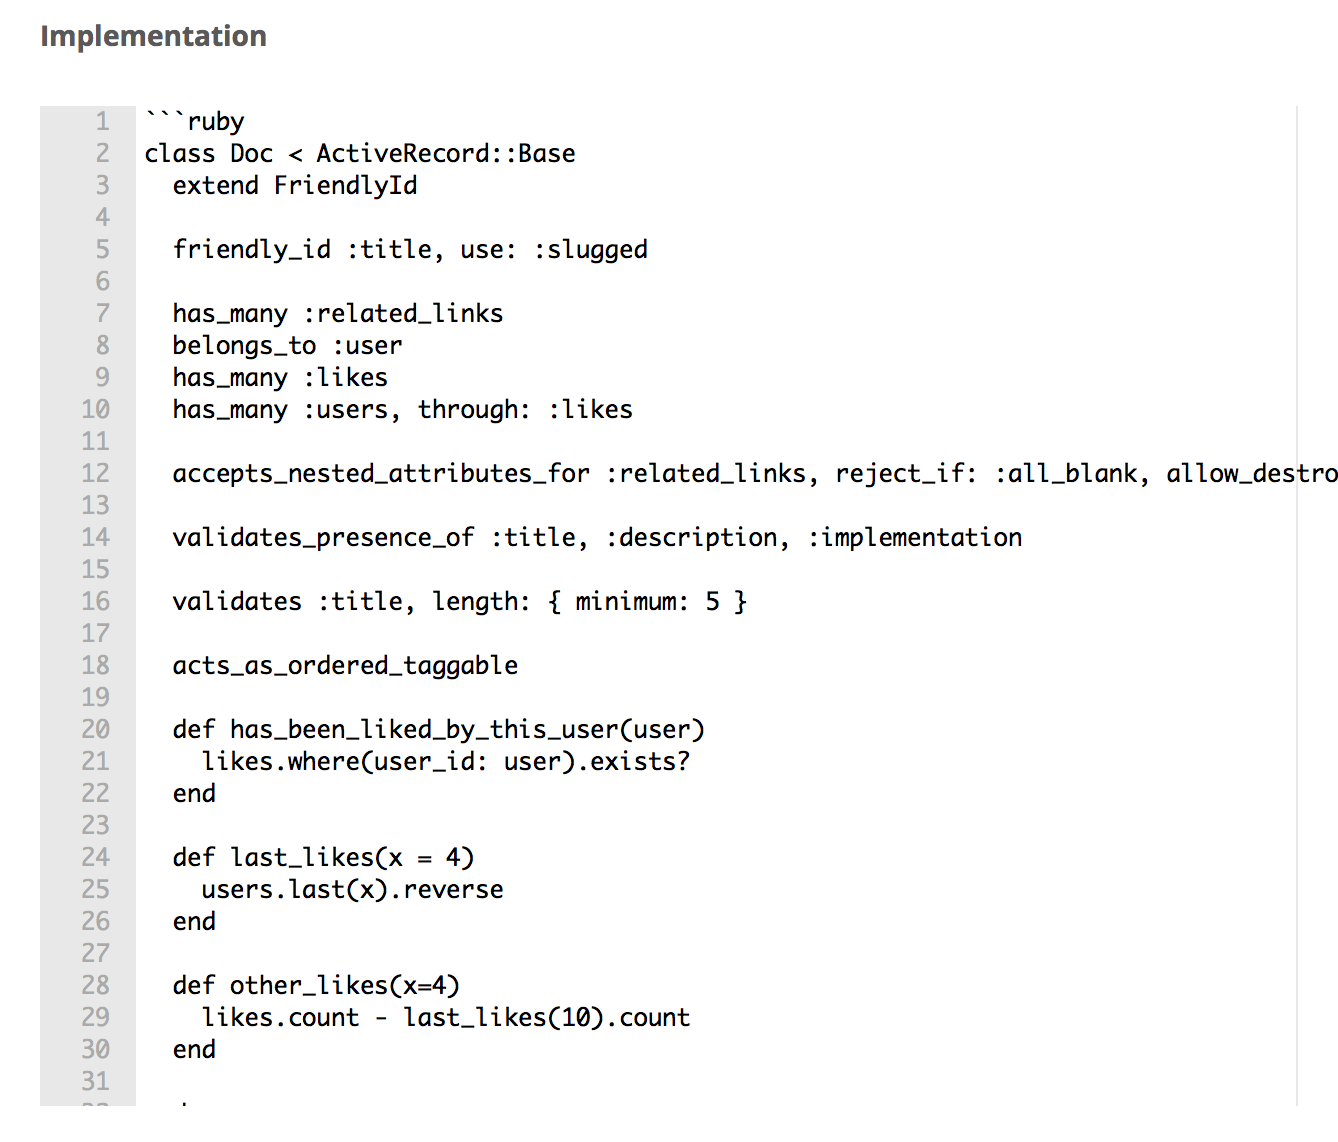
\includegraphics[width=15cm]{Imagens/import-file.png}
		\label{fig:doc-import-1}
	\caption*{Fonte: O autor (2015)}
\end{figure}

\begin{figure}[h!]
	\centering
    \caption{Importação de Linha de Arquivo}
    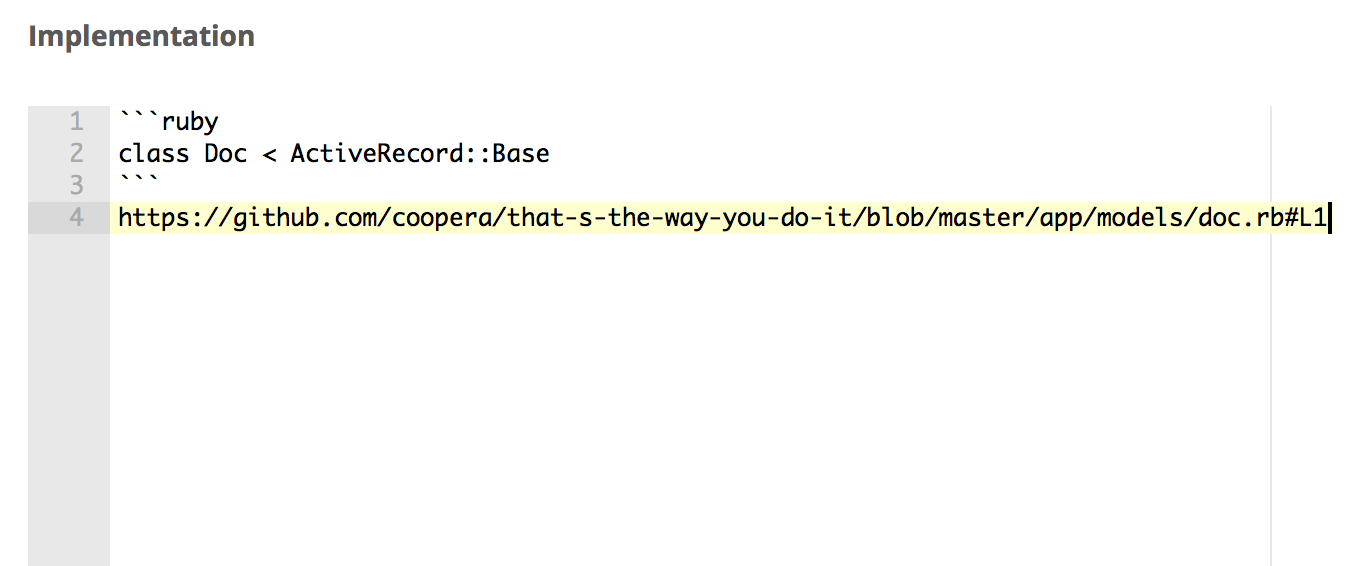
\includegraphics[width=15cm]{Imagens/import-line.png}
		\label{fig:doc-import-2}
	\caption*{Fonte: O autor (2015)}
\end{figure}

\begin{figure}[h!]
	\centering
    \caption{Importação de Múltiplas Linhas de Arquivo}
    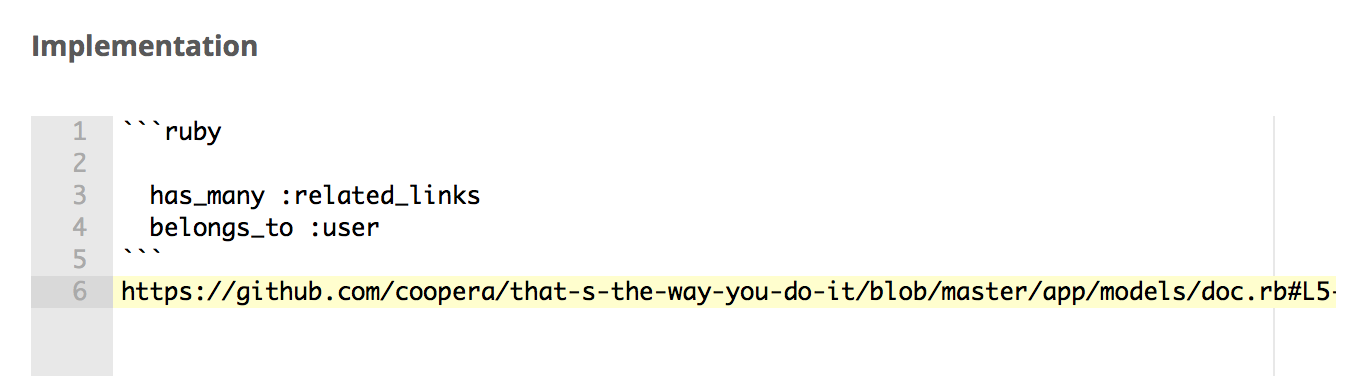
\includegraphics[width=15cm]{Imagens/import-lines.png}
		\label{fig:doc-import-3}
	\caption*{Fonte: O autor (2015)}
\end{figure}

\begin{figure}[h!]
	\centering
    \caption{Importação de \textit{Commit}}
    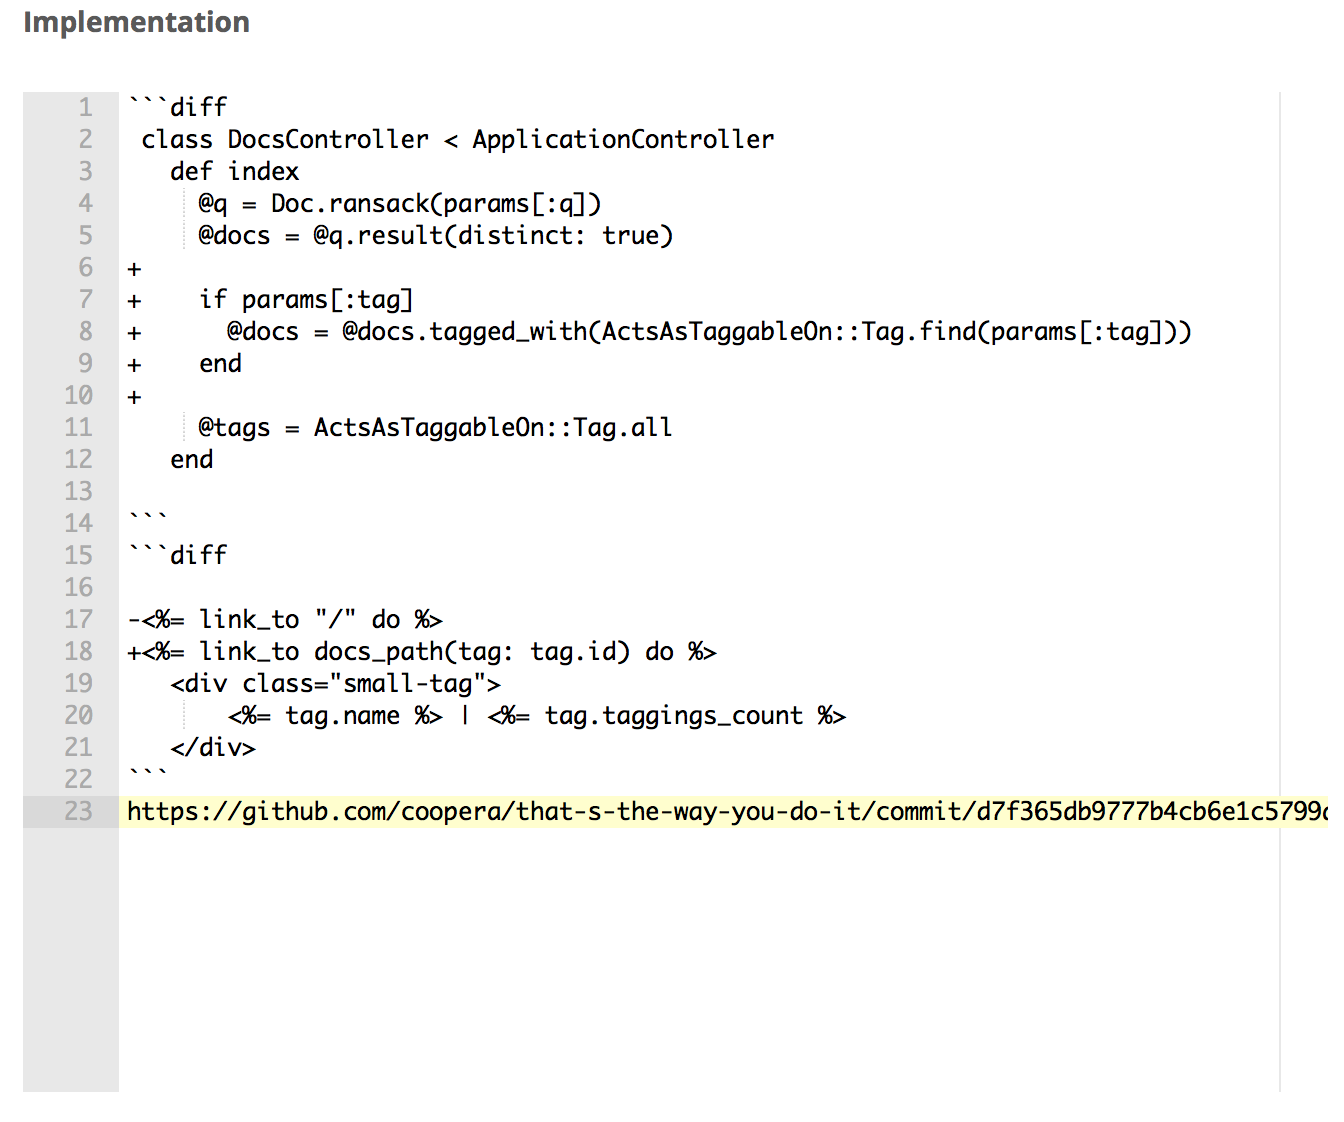
\includegraphics[width=15cm]{Imagens/import-commit.png}
		\label{fig:doc-import-4}
	\caption*{Fonte: O autor (2015)}
\end{figure}

\begin{figure}[h!]
	\centering
    \caption{Importação de \textit{Pull Request}}
    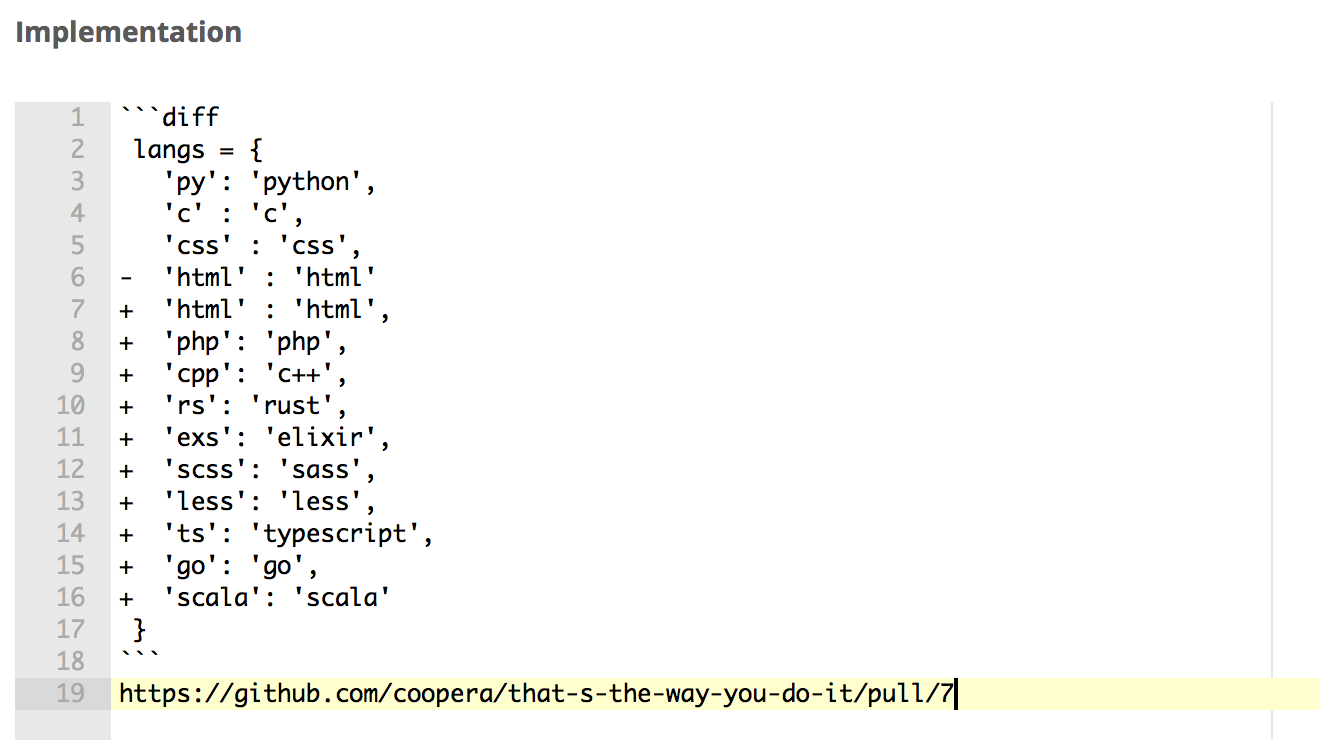
\includegraphics[width=15cm]{Imagens/import-pr.png}
	\caption*{Fonte: O autor (2015)}
\end{figure}

Todo código importado para aplicação já vem formatado como código na linguagem de marcação utilizada. Caso o arquivo importado seja de uma extensão conhecida, é adicionada a marcação para código da linguagem referente àquela extensão. Isso diminui o trabalho do autor para a formatação do texto, permitindo que foque em outros aspectos do documento, como seu texto.

O código importado pode ser livremente modificado, tendo em vista que é texto-puro, permitindo que o autor faça modificações caso ache conveniente.

Além disso, o \textit{link} original colado é mantido para que futuros usuários que consultem o documento possam acessar o código-fonte original disponível no seu respectivo repositório no GitHub.

Sobre a linguagem de marcação utilizada, a próxima subseção a descreve, bem como suas vantagens para o contexto.

\subsection{Suporte a \textit{Markdown}}

Uma linguagem de marcação permite que os autores dos documentos possam formatar seus textos com cabeçalhos, listas, tabelas, entre outros elementos.

Markdown\footnote{\url{https://daringfireball.net/projects/markdown/}} é uma linguagem de marcação amplamente utilizada na web atualmente. Possui sintaxe simples e é utilizada em campos textuais de sites e serviços amplamente utilizados por desenvolvedores de software como os já citados GitHub e Stack Overflow.

Assim, foi optado por adicionar suporte a tal linguagem devido a familiaridade dos desenvolvedores modernos com a mesma.

Dessa forma é permitido aos autores maior clareza e poder de expressão com relação aos documentos criados, além de garantir uma padronização em sua formatação (como de tipografia, por exemplo).

\subsection{Exibição do Documento}

% CITAR FIGURA X, FIGURA Y
Uma vez que o documento é criado, sua visualização fica disponível para todos os usuários. As figuras \ref{fig:doc-show-1}, \ref{fig:doc-show-2} e \ref{fig:doc-show-3} mostram como um documento fica exibido dentro da aplicação.

\begin{figure}[h!]
	\centering
    \caption{Exibição de documento (início)}
    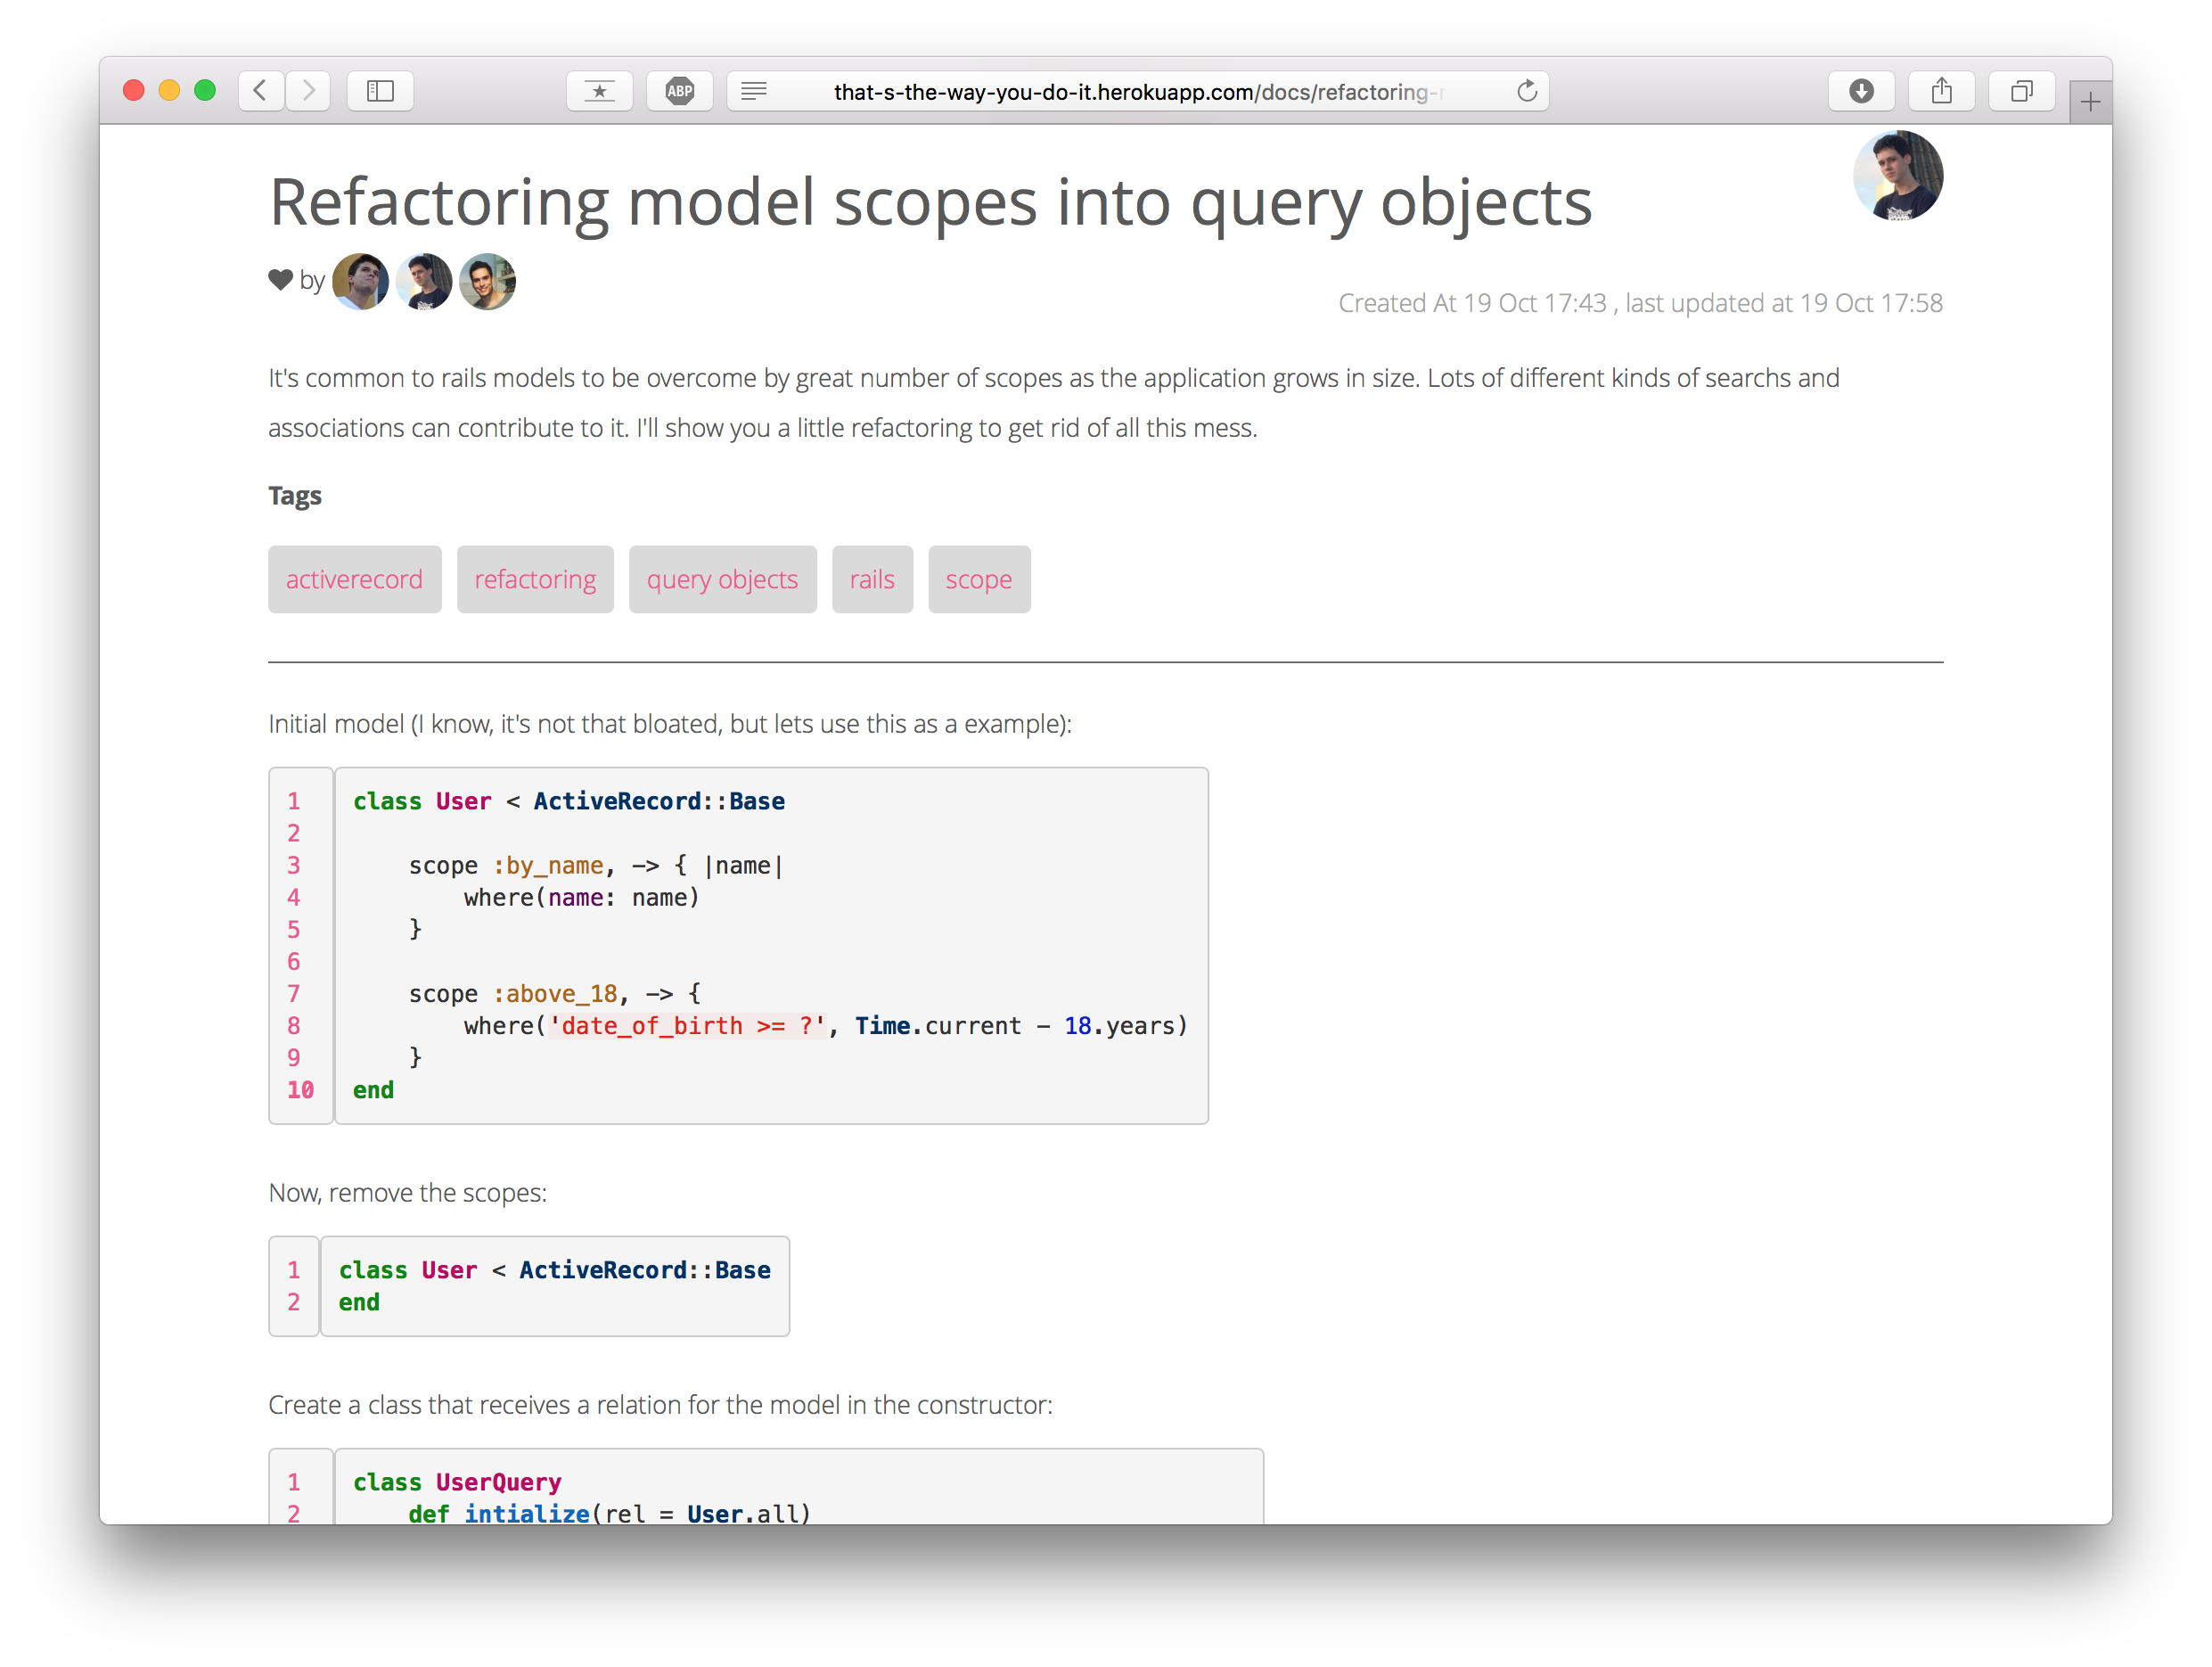
\includegraphics[width=15cm]{Imagens/print-show-1.png}
    \label{fig:doc-show-1}
	\caption*{Fonte: O autor (2015)}
\end{figure}


\begin{figure}[h!]
	\centering
    \caption{Exibição de documento (meio)}
    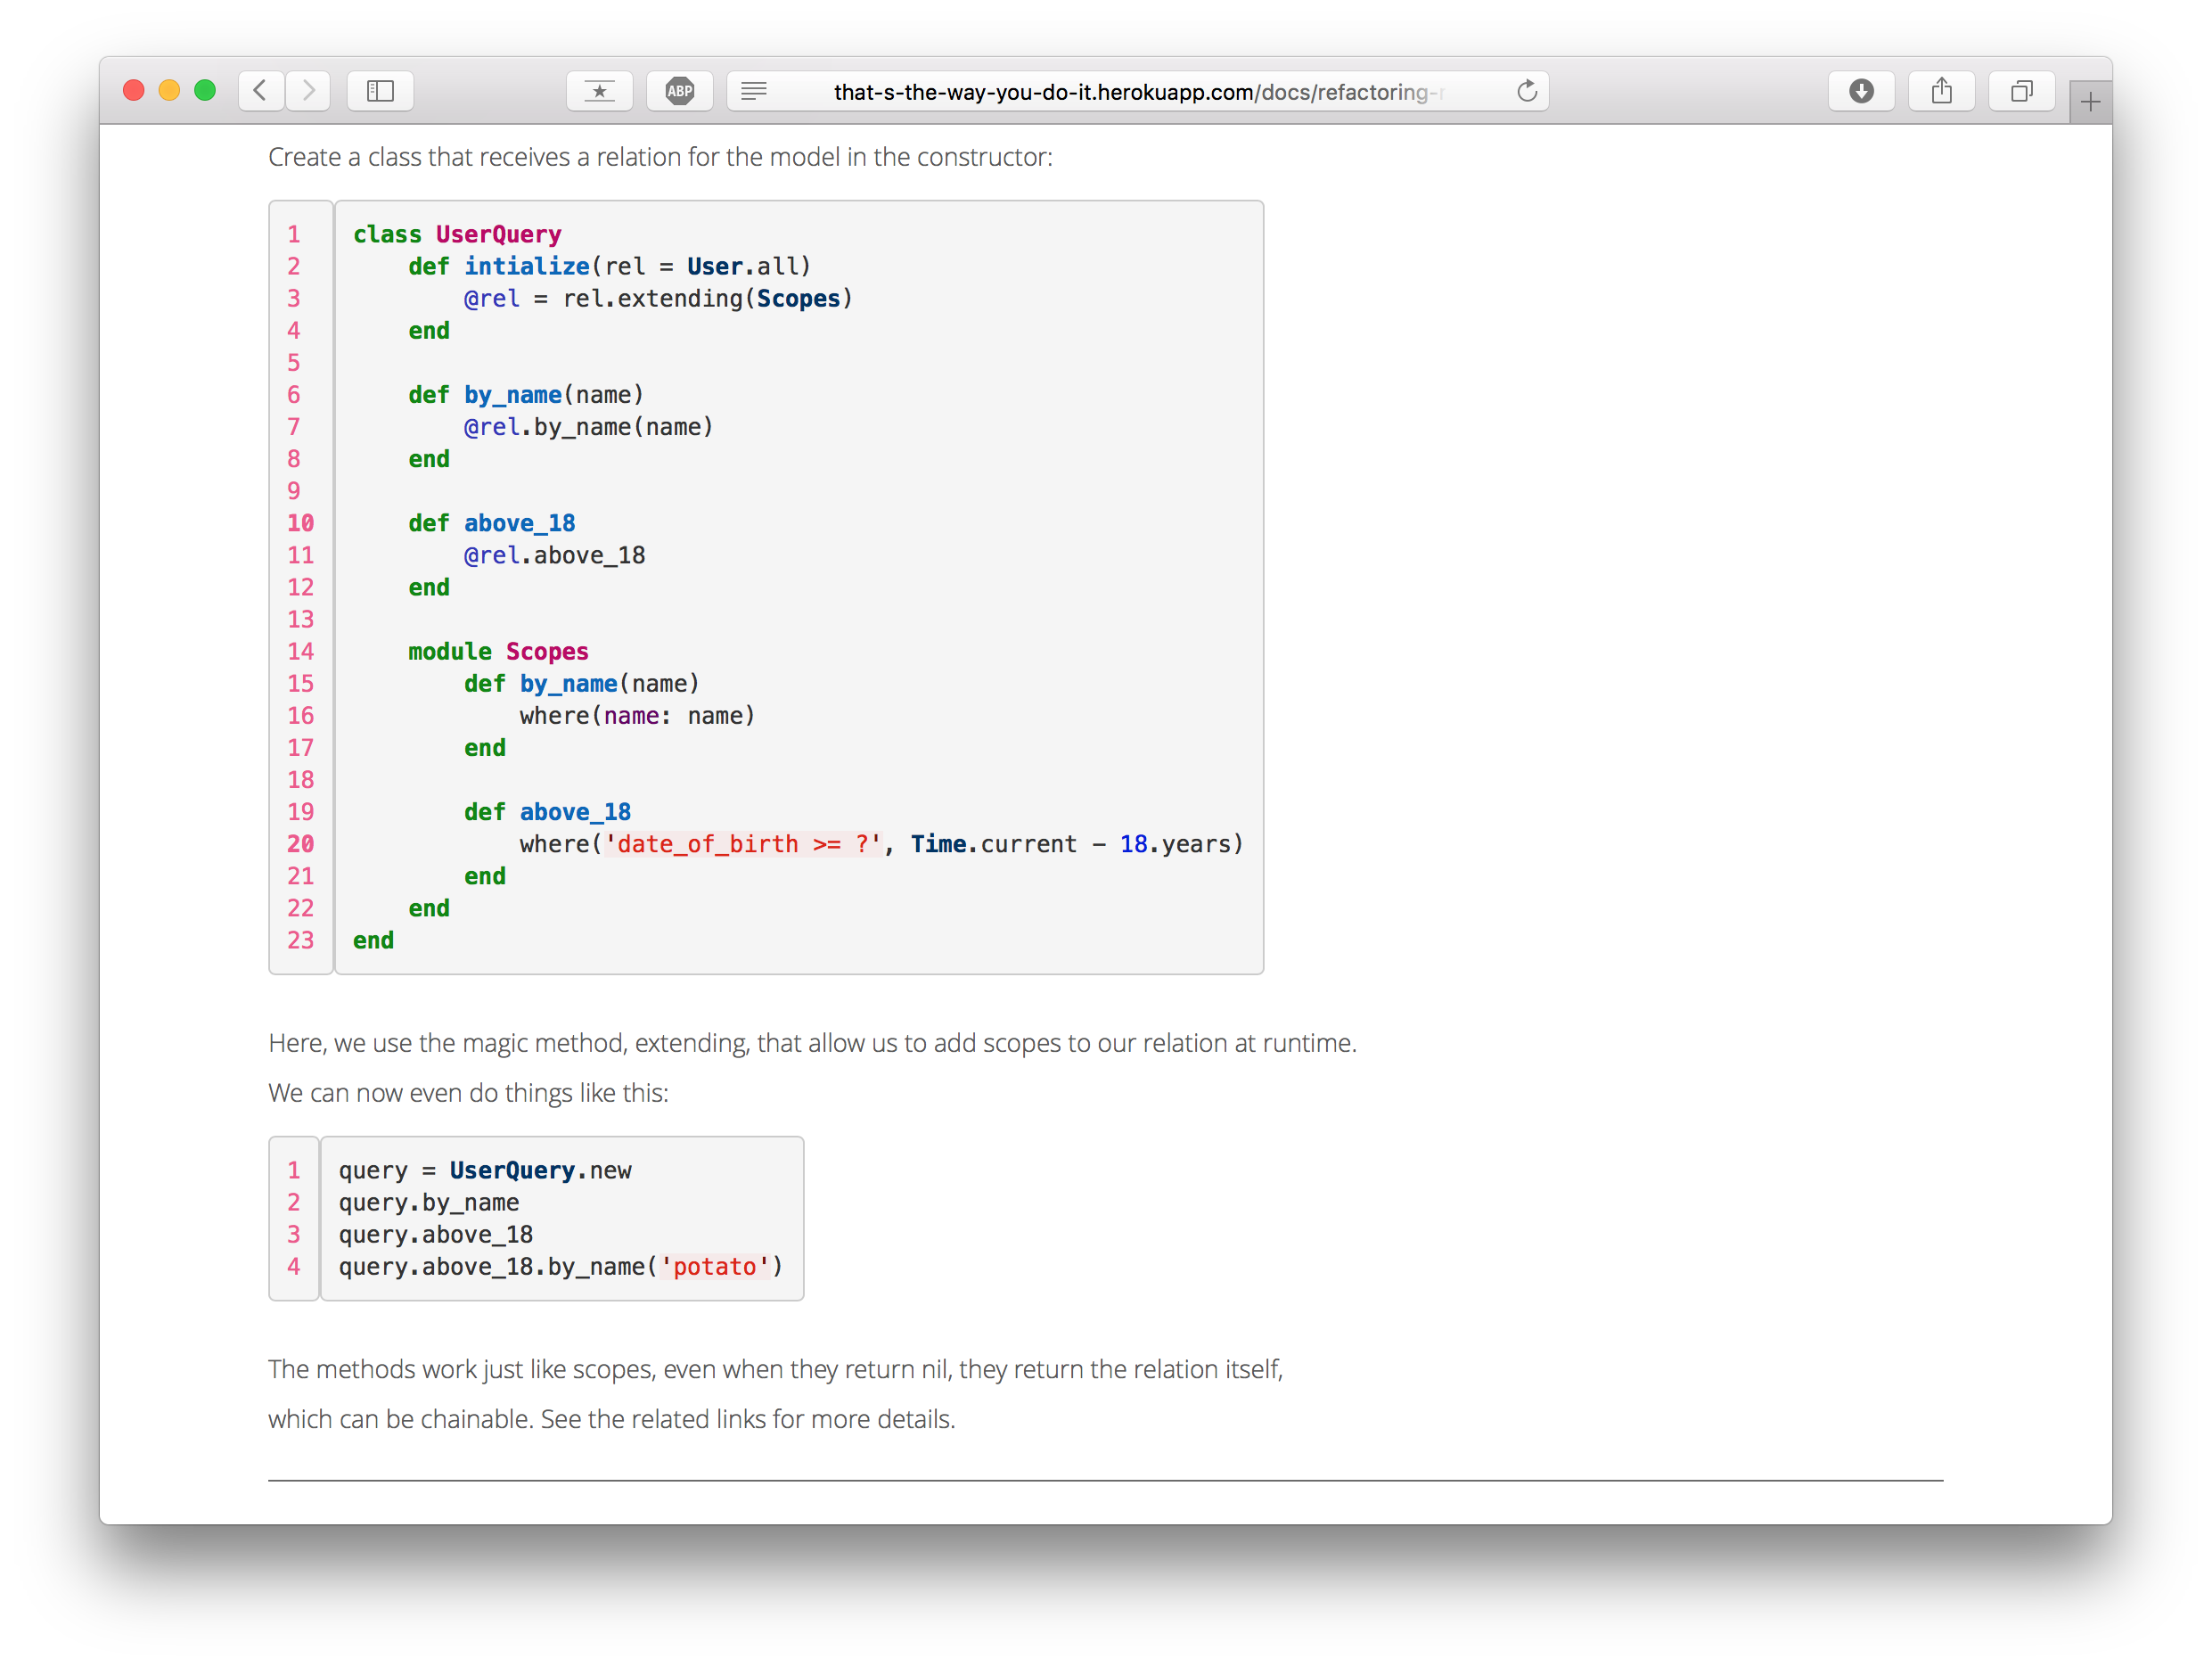
\includegraphics[width=15cm]{Imagens/print-show-2.png}
    \label{fig:doc-show-2}
	\caption*{Fonte: O autor (2015)}
\end{figure}

\begin{figure}[h!]
	\centering
    \caption{Exibição de documento (fim)}
    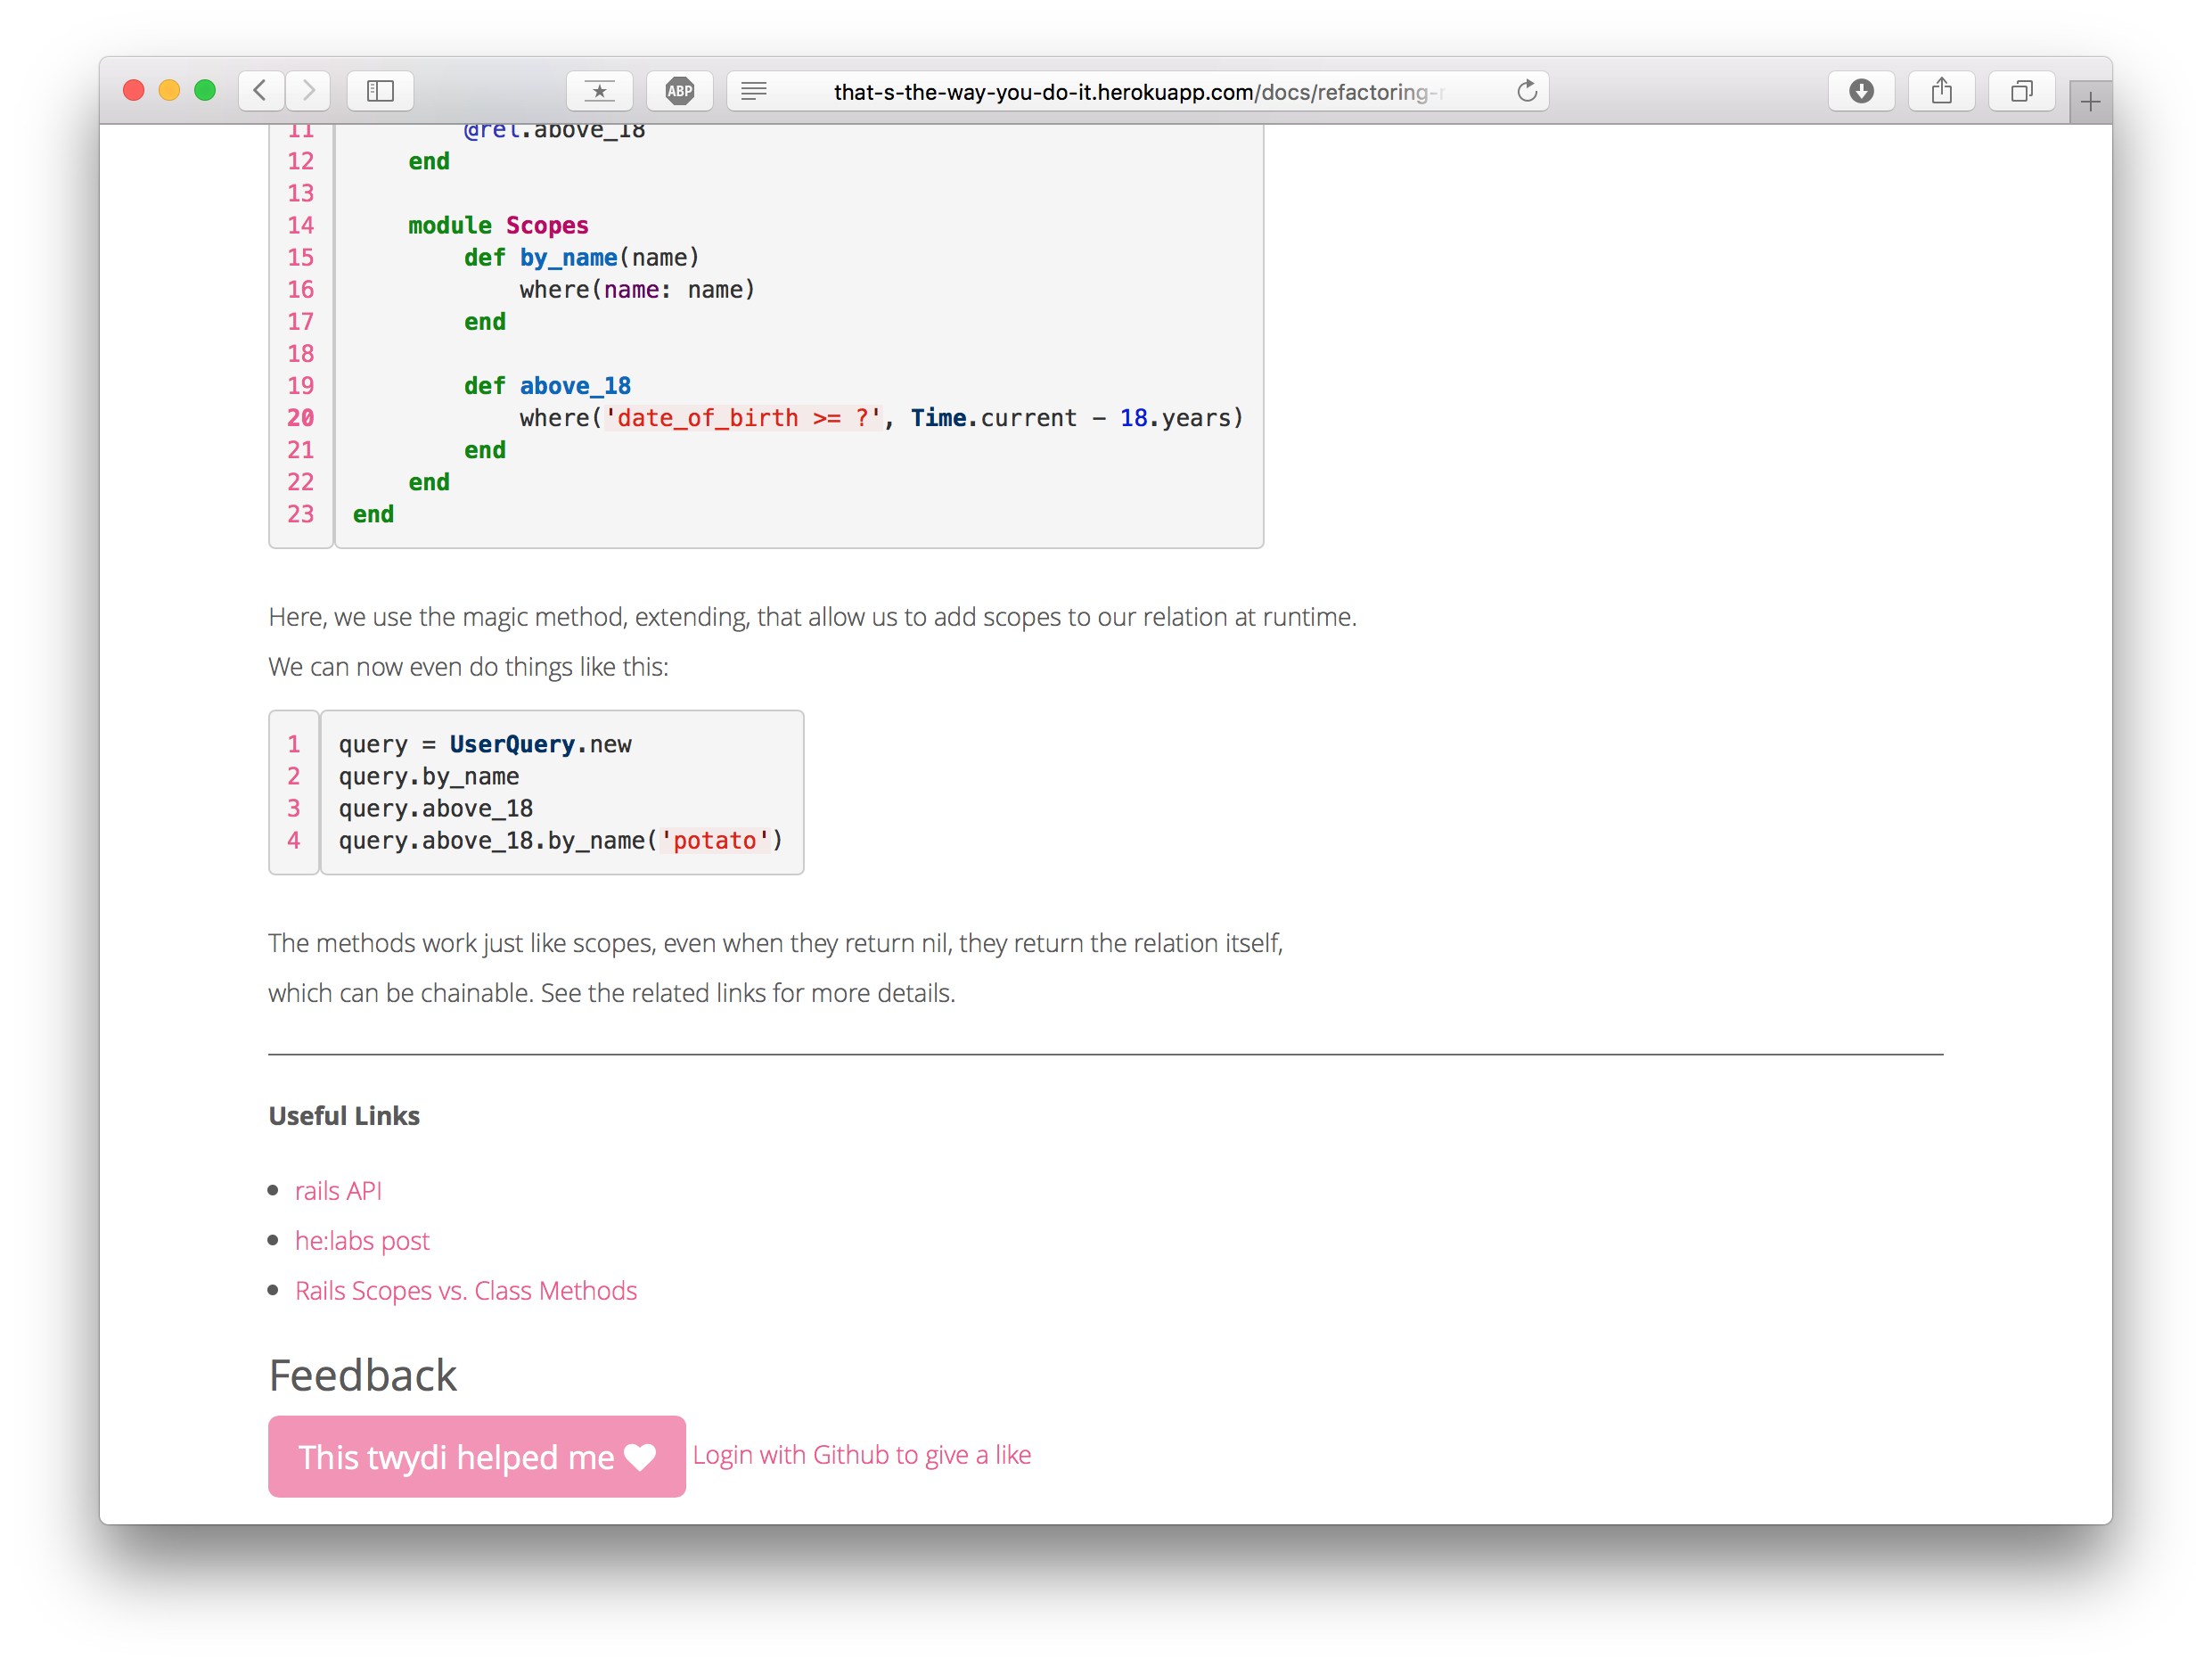
\includegraphics[width=15cm]{Imagens/print-show-3.png}
    \label{fig:doc-show-3}
	\caption*{Fonte: O autor (2015)}
\end{figure}

Enfatiza-se que o elemento de implementação é propriamente renderizado de acordo com a marcação utilizada pelo autor.

\section{Recuperação de Documentos}

Todos os documentos da aplicação são acessíveis por qualquer desenvolvedor. Existem duas formas de fazer esta busca: via \textit{tags} ou via busca textual por algum de seus elementos.

\subsection{Através de \textit{Tags}}

Ao se clicar em uma tag de um documento ou em uma tag presente na lista de tags que se encontra ao fim da lista de documentos, é possível se recuperar todos os documentos que apresentam aquela \textit{tag}.

\subsection{Através de Conteúdo dos Atributos}

Utilizando a barra de busca que se encontra na página que lista todos os documentos da aplicação, é possível realizar uma busca textual que recupera documentos que apresentem o texto informado nos seguintes elementos: Título, Descrição, Implementação ou Links Relacionados.

Além disso, é possível visualizar todos os documentos criados por um usuário ao se clicar no avatar do mesmo em qualquer tela do sistema. Um exemplo da filtragem de documentos por usuário pode ser visualizado na figura \ref{fig:doc-by-user}.

\begin{figure}[h!]
	\centering
    \caption{Lista de documentos de um usuário}
    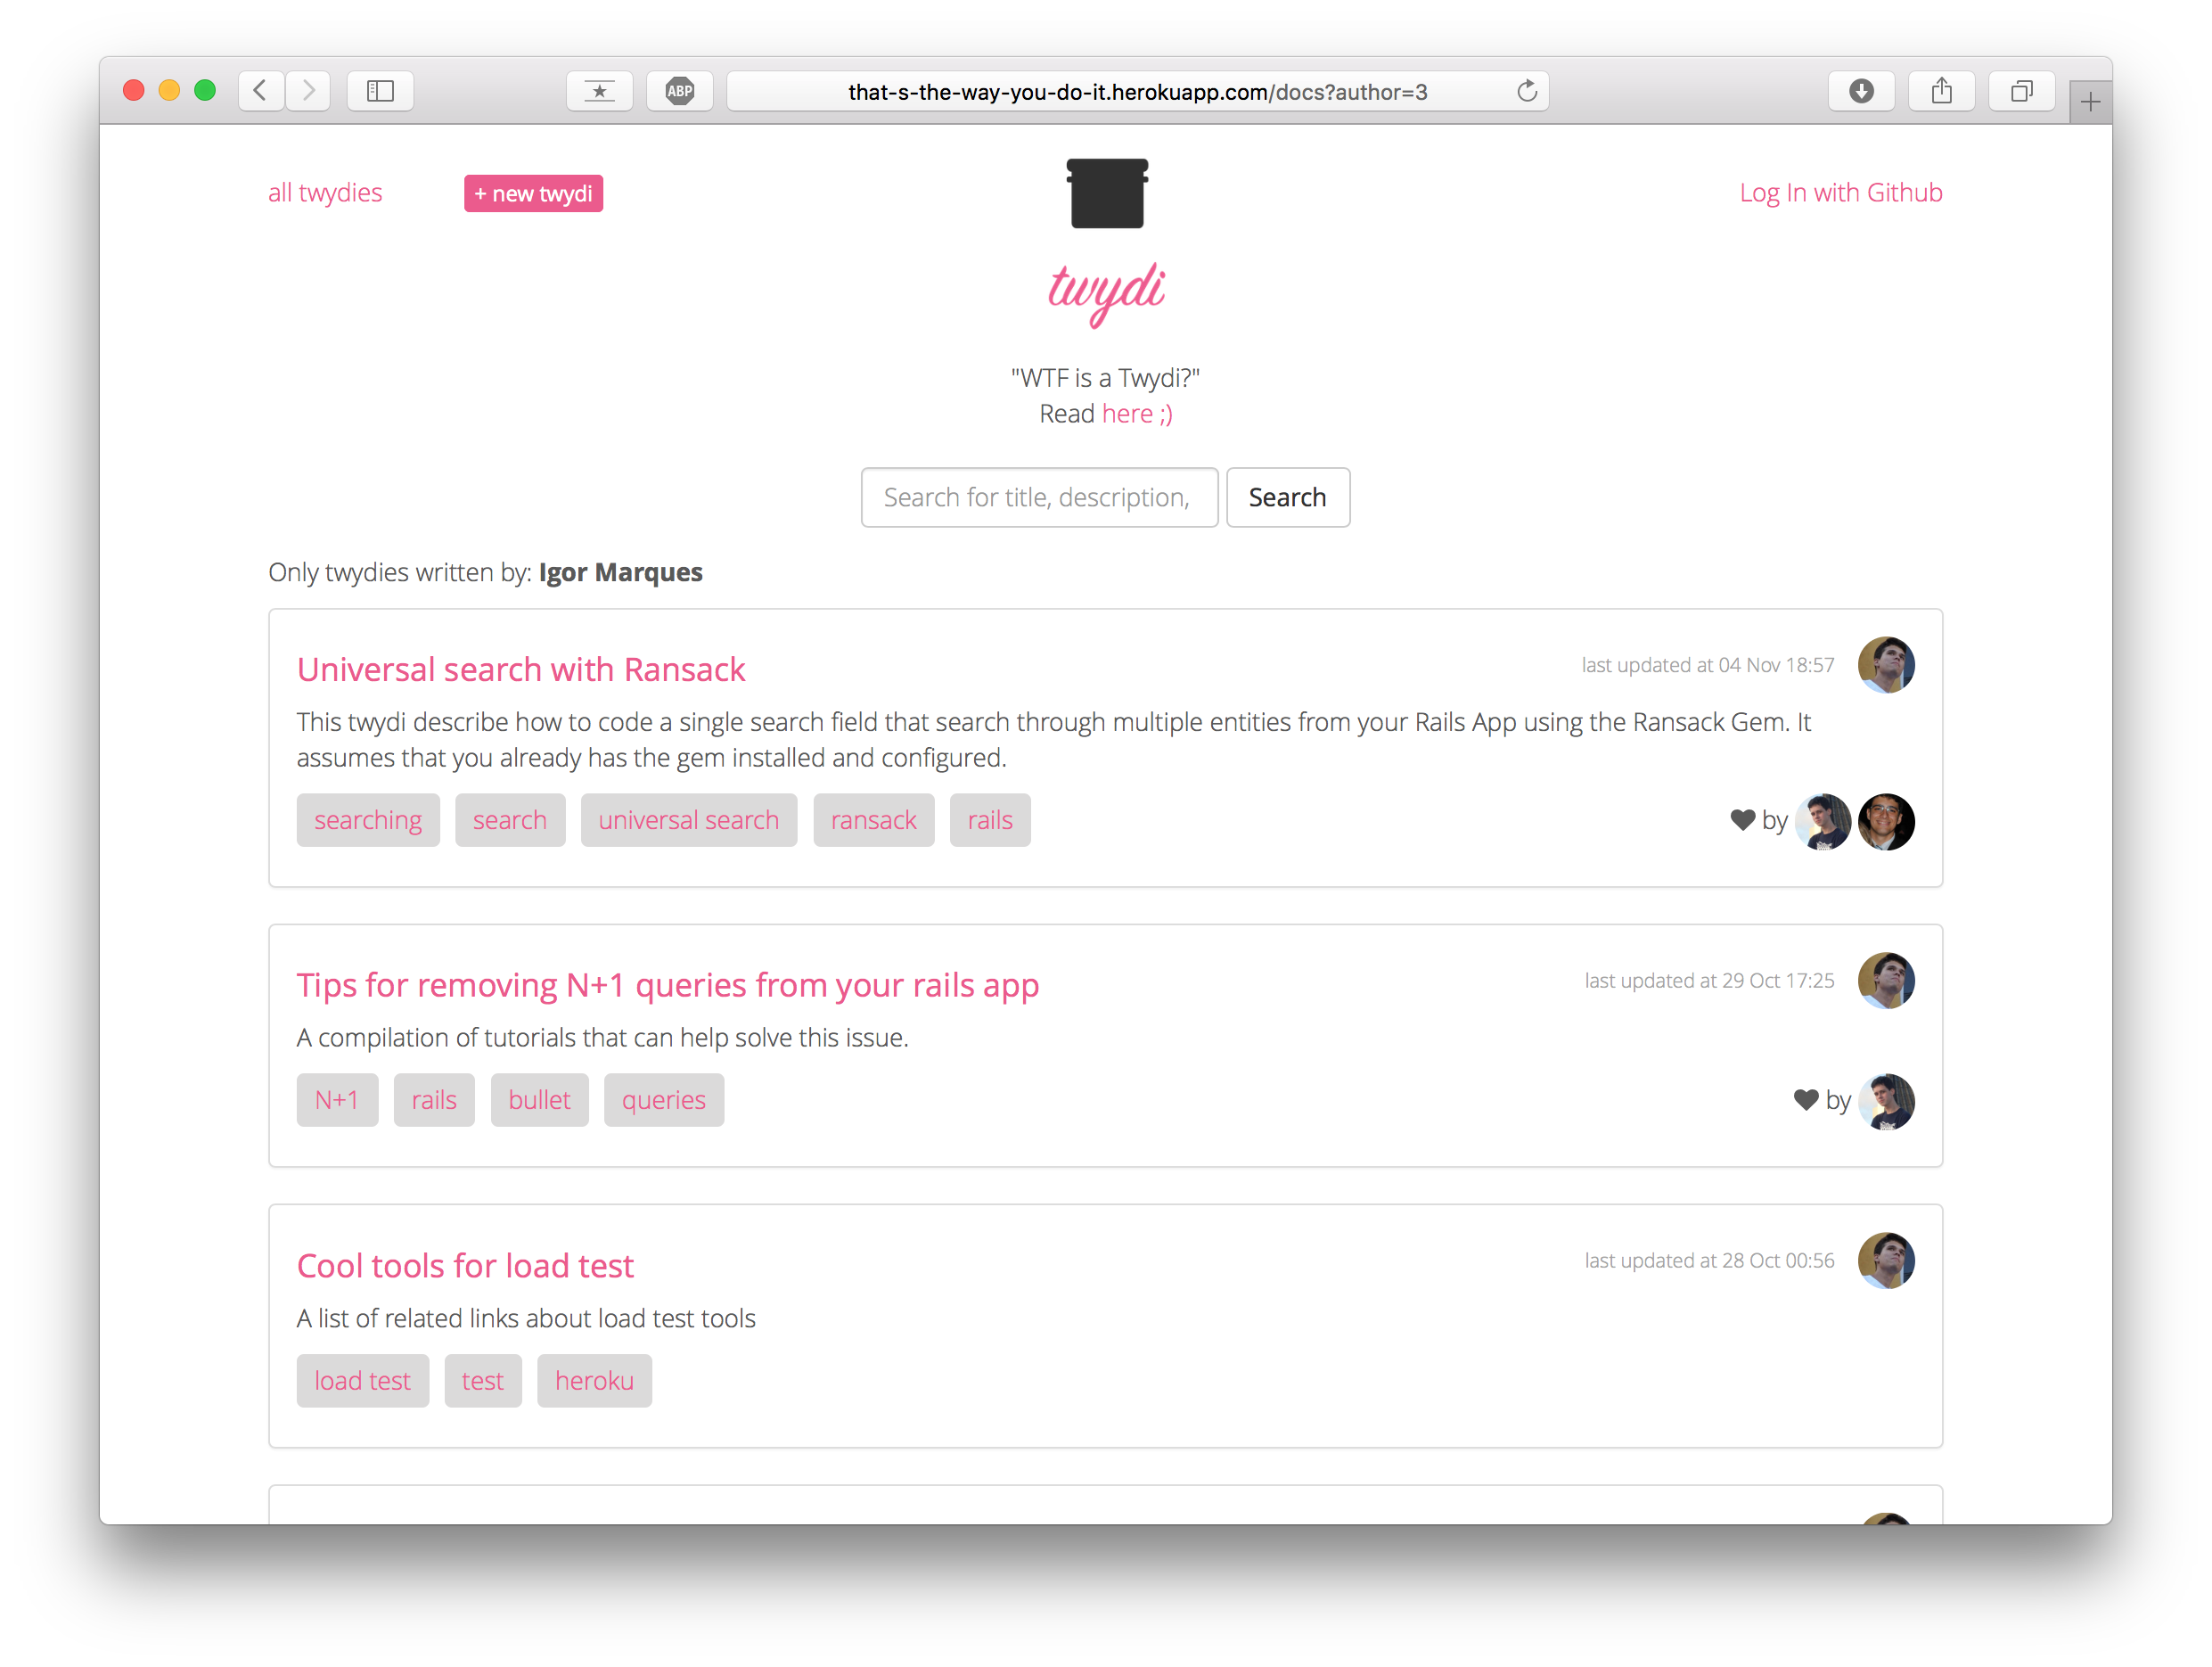
\includegraphics[width=15cm]{Imagens/print-by-user.png}
		\label{fig:doc-by-user}
	\caption*{Fonte: O autor (2015)}
\end{figure}

\section{Autenticação com GitHub}

Para que desenvolvedores sejam identificados como autores dos documentos que criarem, é necessário que se autentiquem na aplicação com sua conta do GitHub. Isso também os permite importar código de repositórios privados para dentro da aplicação, tendo em vista que o GitHub exige autorização do próprio usuário para fornecer código privado.

Além disso, usuários logados podem utilizar a funcionalidade de ``Curtir'' documentos, descrita na próxima seção.

\section{``Curtir'' Documentos}

Usuários autenticados podem utilizar esta funcionalidade, que permite adicionar uma ``curtida'' a um documento. Ao fazer isso, todos os outros usuários da aplicação podem ver que aquele desenvolvedor ``curtiu'' aquele documento tanto na página do documento em si quando na página de listagem de documentos. Figuras \ref{fig:doc-like-1} e \ref{fig:doc-like-2} ilustram a funcionalidade.

\begin{figure}[h!]
	\centering
    \caption{Visualização dos ``Curtir'' em um documento}
    
\includegraphics[width=15cm]{Imagens/print-like-1.png}
		\label{fig:doc-like-1}
	\caption*{Fonte: O autor (2015)}
\end{figure}

\begin{figure}[h!]
	\centering
    \caption{Visualização dos ``Curtir'' na lista de documentos}
    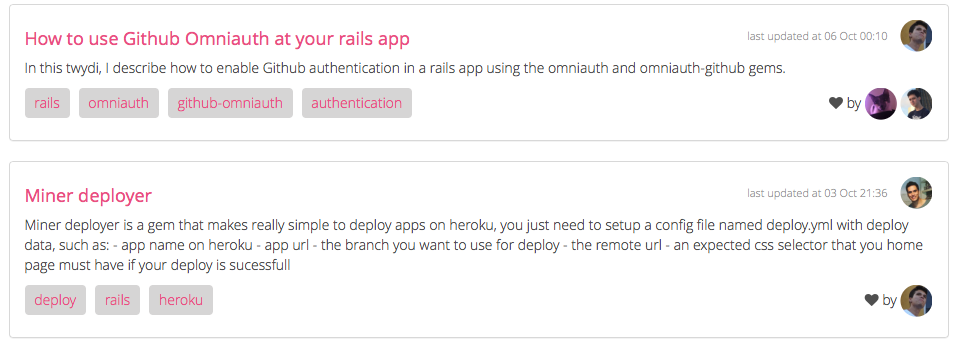
\includegraphics[width=15cm]{Imagens/print-like-2.png}
		\label{fig:doc-like-2}
	\caption*{Fonte: O autor (2015)}
\end{figure}

Esta funcionalidade permite ao usuário informar que o documento curtido foi útil para ele de alguma forma ou que pode ser útil para outros usuários, estimulando sua consulta por estes.

\section{Limitações da Ferramenta}

A aplicação ainda possui algumas limitações em suas funcionalidades. A respeito da importação, a ferramenta não suporta no momento a importação via \textit{links} de código que se encontram em outros ramos (\textit{branches}) de desenvolvimento do repositório.

Além disso, a ferramenta não trata mudanças que possam ter ocorrido na fonte do código importado. Ou seja, uma vez importado, mudanças ocorridas no código disponível no GitHub não se refletem na aplicação.

% IM: falar das vantagens e desvantagens? /\
